\chapter{Background}\label{chap:background}

\todo{Add Glossary?}

\todo{use more formal language}

\todo{write poolmanagers for printing}



Chromatin usually describes different levels of how DNA organizes itself. The
well-known double-helix is only the lowest of several structural layers.
Looking at it from the outside (highest structural layer), DNA looks similar to
a big ball of wool. With the help of chromosome conformation technologies
spatial proximity can be visualized


\section{Chromosome Conformation Technologies}\label{sec:cct}


\begin{figure}[t]
\begin{centering}
    {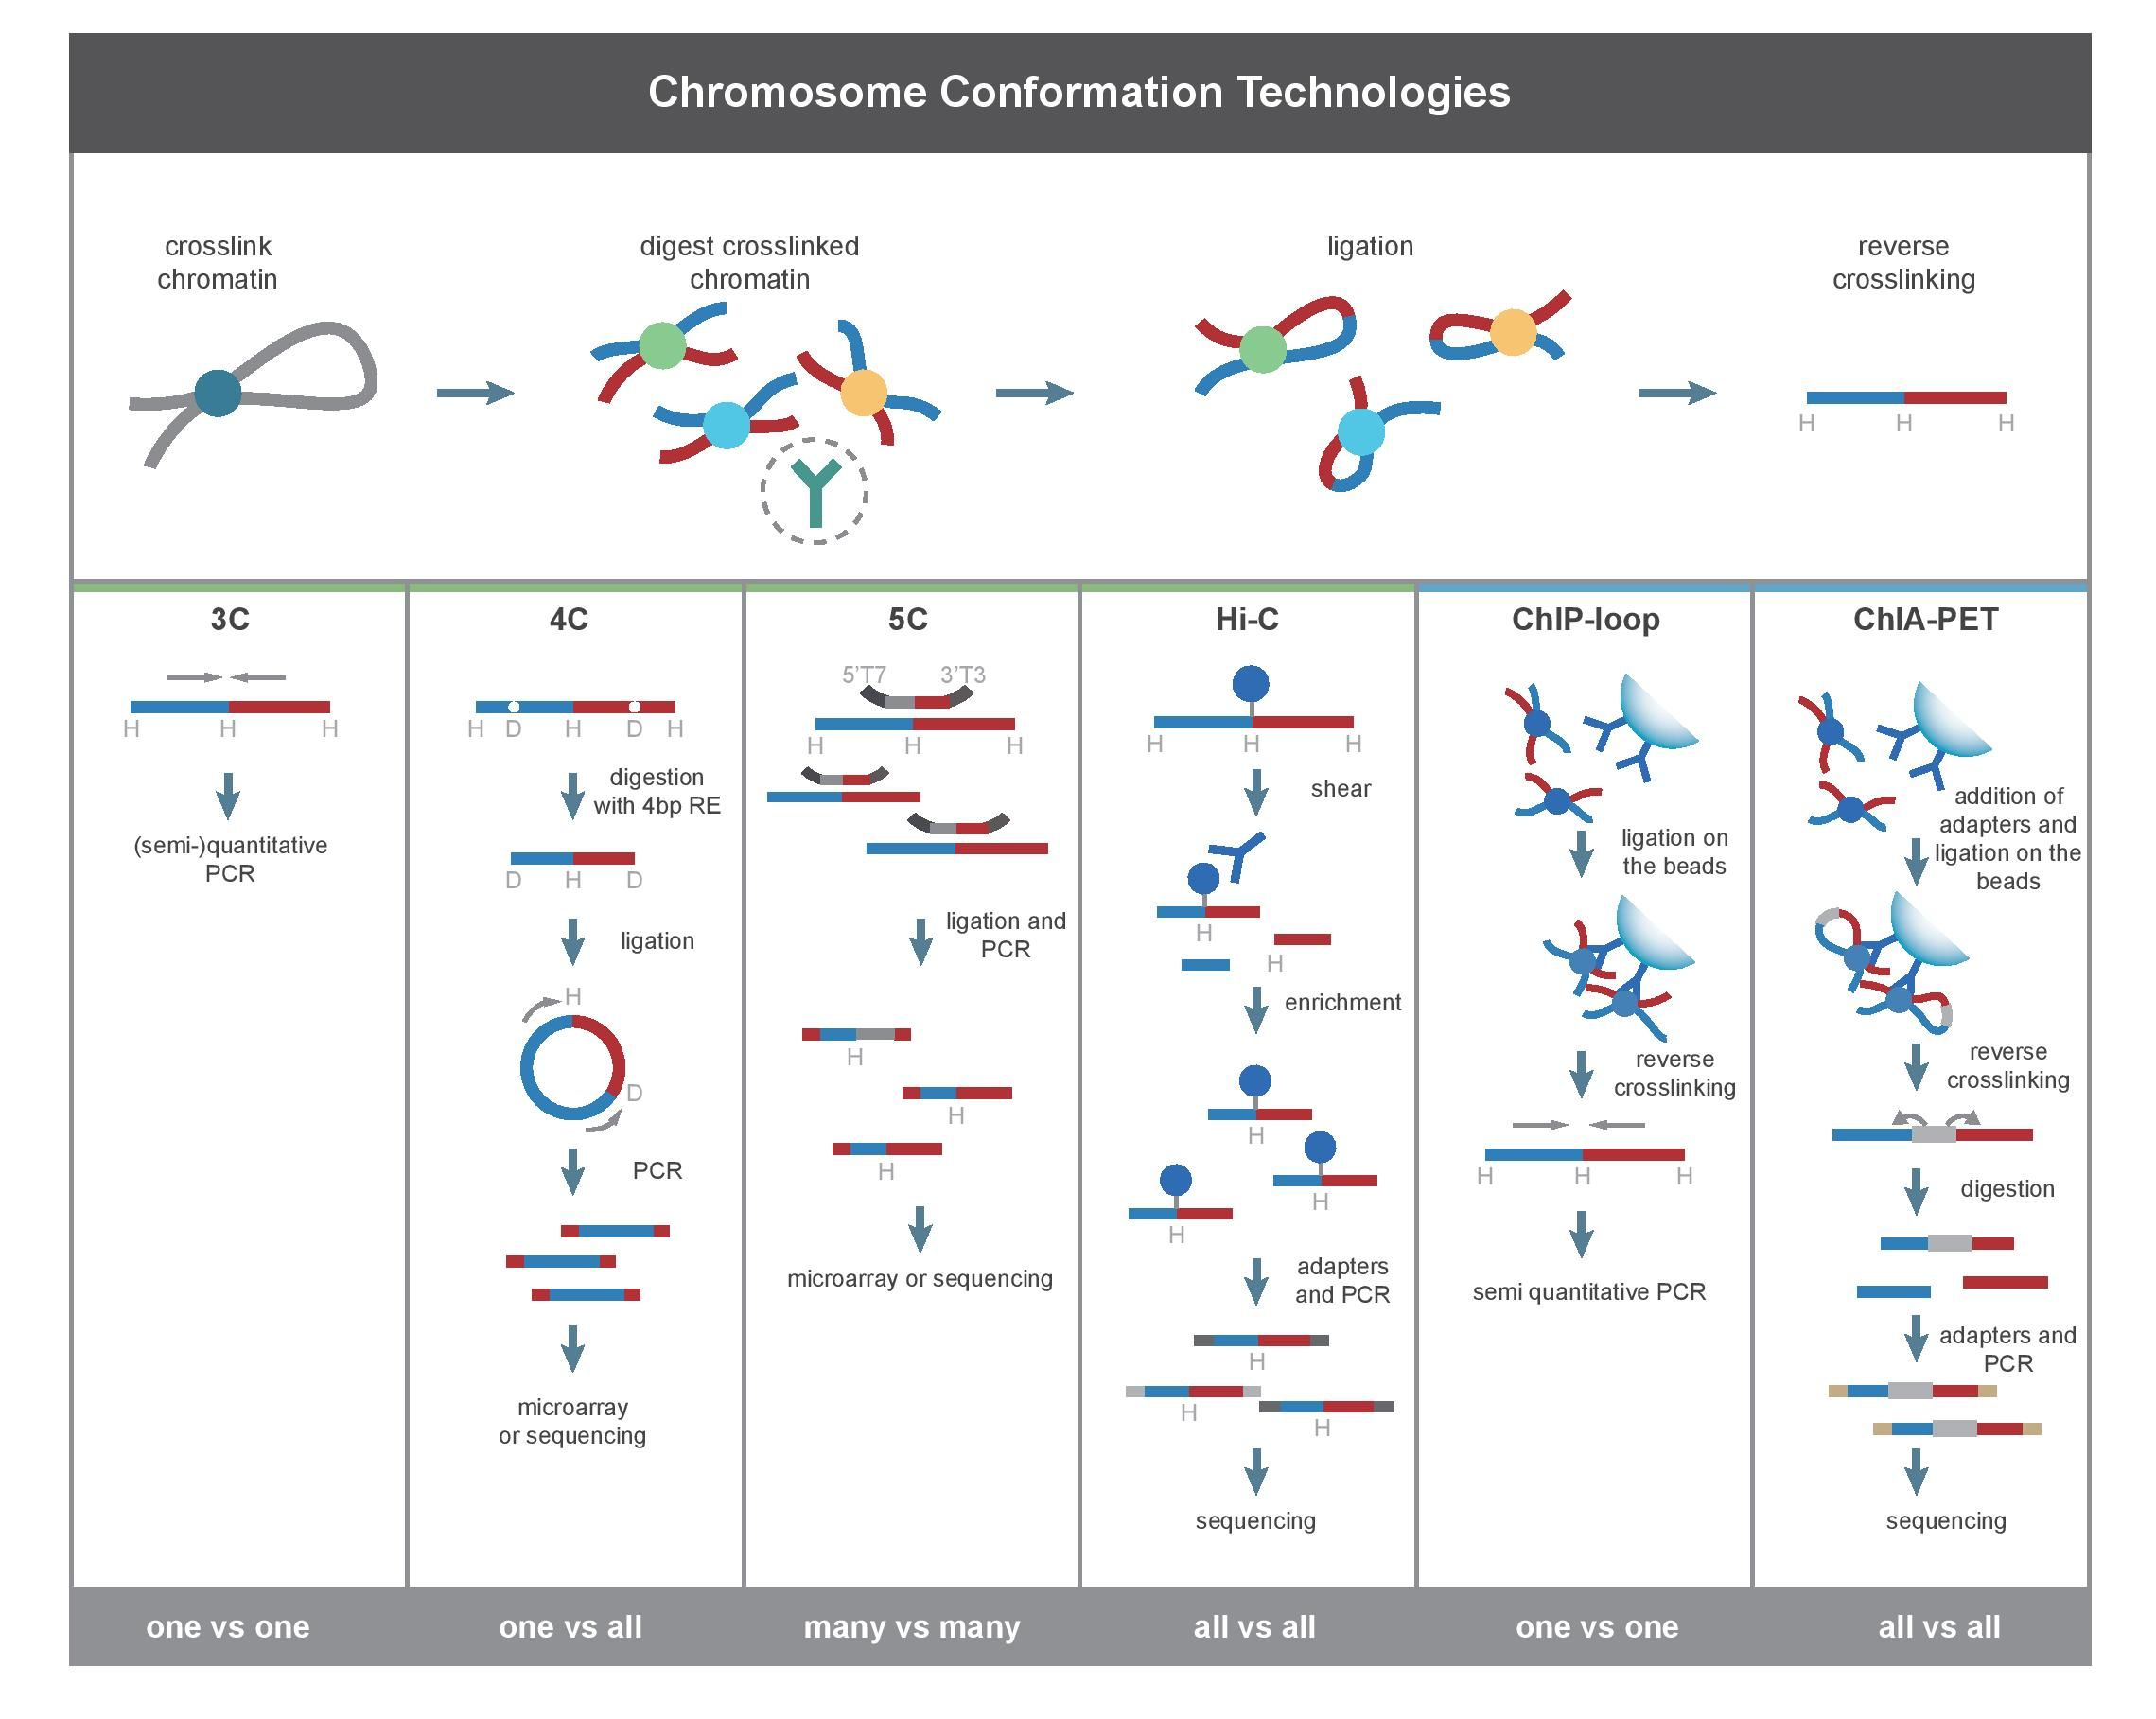
\includegraphics[scale=0.75]{figures/background/Chromosome_conformation_techniques.jpg}}
    \caption[Comparison between 3-C and its derived methods]
    {\textbf{Comparison between 3-C and its derived methods.}
    Clearly seen can be why 3-C, 4-C, 5-C and Hi-C are commonly referred to as
    3-C-based techniques.
    % ChIP-loop and ChIA-PET have these steps in a modified
    % version as well.
    \\ \\ Image from \cite{Li2014}.}
    \label{fig:comparison3C}\label{fig:cct}
\end{centering}
\end{figure}





\subsection{Common steps}\label{sec:common}

As can be seen in \figref{fig:cct}, The first steps, crosslinking, digestion,
ligation and the reversal of crosslinking, are the same for all 3-C-based methods.

\subsubsection{Cross-linking DNA}\label{sec:crosslinking}

The first step is to cross-link DNA strands that are close to each other
spatially (see \figref{fig:cct} or \figref{fig:HiC} for reference). This is done by adding
formaldehyde, which connects (links) sufficiently close strands together.

A chromatin cross-link is two entirely different parts of the genome held
together by a chemical bond with formaldehyde. This process cannot be
specifically controlled, so only `regions near each other' are connected, but
not necessarily all regions that are known to be spatially close.

\subsubsection{Digestion}\label{sec:digestion}

The next step is cutting the DNA, currently more similar to a ball of wool,
apart in intervals. For this, restriction-enzymes are used (specifically
restriction endonuclease). Commonly used enzymes for this are DpnII or HindIII,
cutting the genome every 4000 base-pairs \cite{liebermann2009comprehensive}.
This will result in a lot of cross-linked fragments, as well as
not-cross-linked ones.

\subsubsection{Ligation}\label{sec:ligation}

After reducing the concentration of fragments, DNA ligase is added, to ligate
(weld together) dangling fragment ends. For this a reduction in concentration
is done since mostly fragments close together are ligated, it is intend to
ligate fragments linked together by formaldehyde.

In HiC, Biotin is added in this step to mark ligated fragments. This allows
filtering out most fragments that have not been ligated in a later step.


\subsubsection{Reverse Cross-links}\label{sec:revcrosslink}

% Source: http://www.protocol-online.org/biology-forums/posts/10475.html
Adding a high concentration of salt for some time will reverse the
cross-linking through formaldehyde, leaving us with our two originally
spatially close fragments ligated and with a biotin-marker.


Note that at this point, the fragments are too long to sequence them.
They are ligated fragments of around 8000 base-pairs, but most current
sequencing methods can only deal with sequence lengths of a few hundred
base-pairs at most.




\subsection{3-C}\label{sec:3C}

In 2002 Dekker et al. \cite{dekker2002capturing} developed a method test for interactions
between a single pair of genomic loci. Candidates for promoter-enhancer
interactions can be tested using this method.
After the reversal of cross-links (\secref{sec:revcrosslink}), the fragments
\extend{what is (semi-)quantitive PCR?}



\subsection{4-C}\label{sec:4C}

Chromosome conformation capture-on-chip (4C) was developed in 2006 by Simonis,
Zhao et al. \cite{simonis2006nuclear} \cite{zhao2006circular}, a method to test
interactions between one genomic loci to all others. This is done by adding a
second ligation-step (see \secref{sec:ligation}, \figref{fig:cct} for
reference) creating loops from the DNA fragments and applying inverse-PCR
(method to specifically amplify the unknown parts when beginning and ending
parts are known, for this the loops are cut within the known section).
Afterwards, this may get sequenced. Due to inverse-PCR knowledge about both
interacting chromosomal regions is not needed.  Results are highly reproducible
for close regions \draft{find source for this}.

\extend{What is a microarray?}



\subsection{5-C}\label{sec:5C}

Chromosome conformation capture carbon copy (5C) was developed in 2006 by
Dostie et al. \cite{dostie2006chromosome}, this method is able to test a region
for interactions with itself, such region being no bigger than a megabase. This
is done by adding universal primers to all fragments from such a region.
5-C has relatively low coverage, but is useful to analyse complex interactions
of specified loci of interest. Genome-wide interaction measuring would require
millions of 5C primers, making this method unsuitable.



\begin{figure}[t]
\begin{centering}
%    \subfloat[Diagram summarising the Hi-C experimental protocol. The red and blue rectangles represent cross-linked restriction fragments while the yellow marker shows the position of biotin incorporation.]
%    \subfloat[Generation of the Hi-C ligation junction sequence by successive digestion (with HindIII in this example), fill in and blunt-ended ligation steps. The modified restriction site sequence is not found in the original genomic sequence.]
    {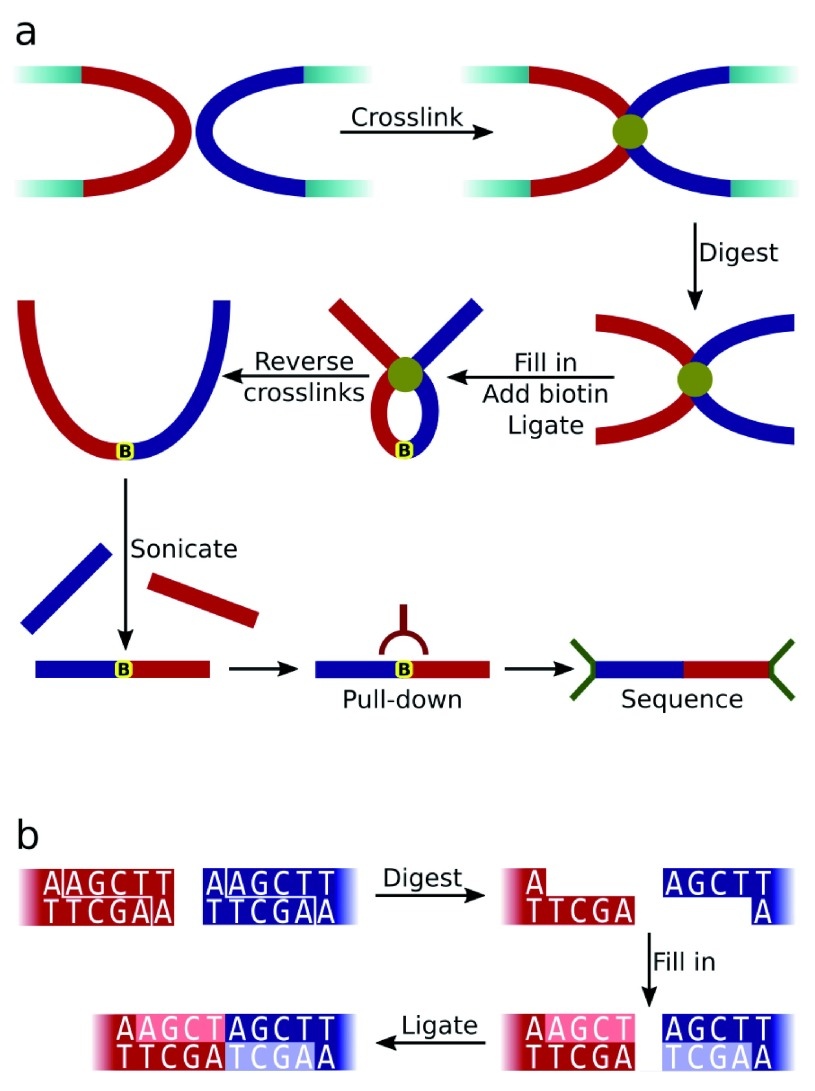
\includegraphics[scale=4]{figures/background/f1000research-4-7903-g0000.jpg}}
    \caption[Summarised Hi-C protocol]
    {\textbf{a)} Diagram summarising the Hi-C experimental protocol. The red and blue rectangles represent cross-linked restriction fragments while the yellow marker shows the position of biotin incorporation. \textbf{b)} Generation of the Hi-C ligation junction sequence by successive digestion (with HindIII in this example), fill in and blunt-ended ligation steps. The modified restriction site sequence is not found in the original genomic sequence. \\ \\ Image and description taken from \cite{wingett2015hicup}.}
    \label{fig:HiC}
    \todo{rewrite the description in my own words}

    \todo{remove the b section}
\end{centering}
\end{figure}



    % {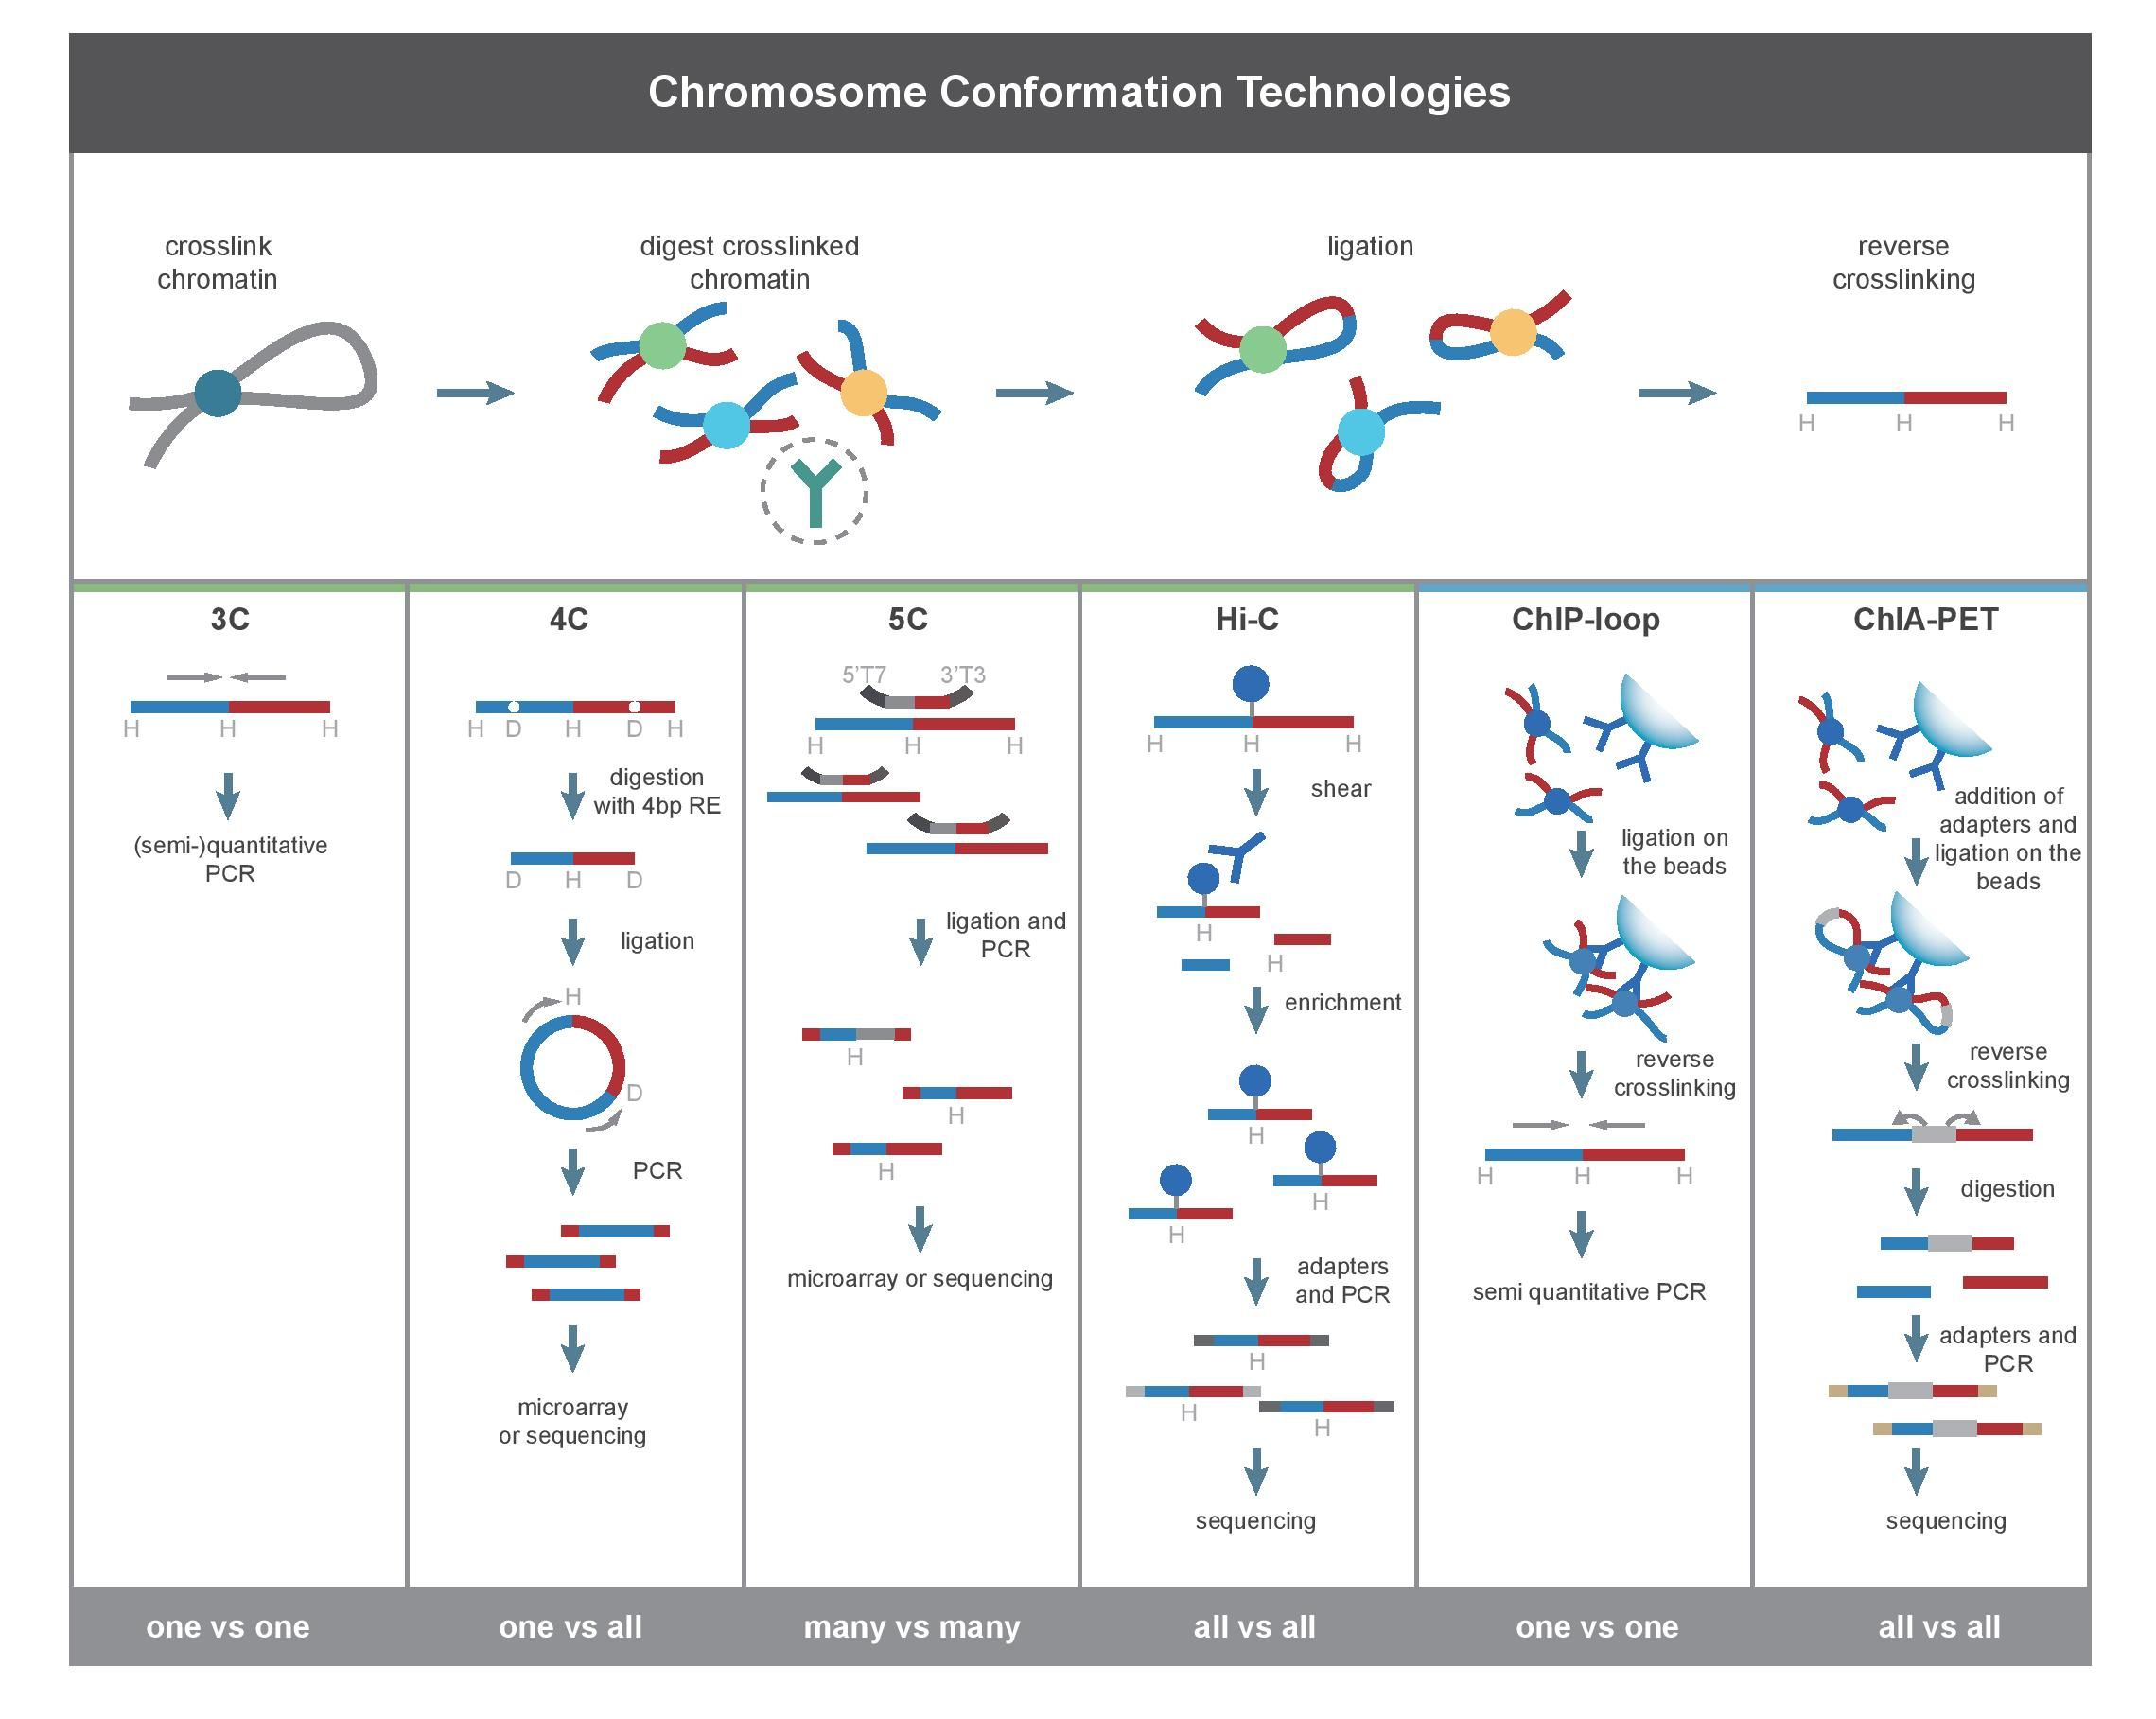
\includegraphics[scale=0.8]{figures/background/Chromosome_conformation_techniques.jpg}}
    % \caption[Comparison among 3C and its derived methods]{\textbf{Comparison among 3C and its derived methods} Source: https://en.wikipedia.org/wiki/File:Chromosome\_conformation\_techniques.jpg}




\subsection{Hi-C}\label{sec:HiC}

Hi-C (as shown by \figref{fig:HiC}) was developed in 2009 by Liebermann-Aiden et al.
\cite{lieberman2009comprehensive}. After the common steps noted earlier, unique
to Hi-C is the following sequence of sonication, pulldown (filtering based on
biotin markers) and sequencing.


\subsubsection{Sonication}\label{sec:sonication}

Putting the ligated DNA-fragments under the influence of ultrasonic waves is
breaking them apart in much shorter fragments (due to long sequences not being
able to absorb frequent shocks well), shearing them apart in sequences short
enough to enable sequencing.


\subsubsection{Filtering and Removal of Biotin}\label{sec:pulldown}

`pulling-down' fragments marked with biotin leaves only those having been
marked, and thus ligated, earlier (see \secref{sec:ligation}). Subsequently the
marker is removed, as it would hinder further sequencing.

\subsubsection{Sequencing}\label{sec:sequencing}

Sequencing, short for DNA sequencing, describes processes of measuring a DNA
sequence. There are several techniques for doing this, most use PCR (Polymerase
Chain Reaction) before or while sequencing, which duplicating fragments
several times, allowing them to be sequenced more accurately.

% - putting the 3' and 5' ends there
% - usual PCR methods


% Hi-C (all-vs-all)
% Hi-C uses high-throughput sequencing to find the nucleotide sequence of
% fragments.[2][22] The original protocol used paired end sequencing, which
% retrieves a short sequence from each end of each ligated fragment. As such,
% for a given ligated fragment, the two sequences obtained should represent two
% different restriction fragments that were ligated together in the random
% ligation step. The pair of sequences are individually aligned to the genome,
% thus determining the fragments involved in that ligation event. Hence, all
% possible pairwise interactions between fragments are tested.


% Researchers attempt to study the extent of Hi-C's detection through a study
% focusing on screening primary brain tumours.[30] Prior to screening tumours,
% Hi-C was primarily focused on cell lines.[31]


\subsection{Other methods}\label{sec:other3c}

Other methods, such as ChIP-loop or ChIA-PET exist, however as the are
different from the digestion step onwards, and their subsequent steps are
fundamentally different, they will not be covered in depth.

\draft{explain them at least somewhat, reference to some other source}




% Chromatin is packaged into three-dimensional structures, that retain a
% relationship between genomic and physical distance. Sequences that are closer
% on the same chromosome, are also closer in physical space. Our method
% exploits this relationship between linkage and proximity to enable whole
% chromosomes scaffolding and phasing of genomes.
%
% The DNA in the sample is cross-linked in-vivo to fix DNA sequences present
% inside the same cell. Cross-linking trap sequence interactions across the
% entire genome and between different chromosomes.
%
% Cross-Linked DNA is fragmented with endonucleases. Fragmented loci are then
% biotin elated and ligated creating chimeric junctions between adjecent
% sequences. This process is called proximity ligation.
%
% The more often two sequences are joined together, the closer these two
% sequences are in genomic space.
%
% Biotinylated junctions are purified and subjected to paired-end sequencing.
% The proximity-ligation-reads are then mapped onto a draft assembly.
%
% Proximity information is used to assign context to chromosomes, and order and
% orient them along chromosome scale scaffolds.
%
% This results in fully scaffolded chromosomes of virtually any size. This
% process also detects structural variation and corrects assembly miss-joins as
% well as maps the three-dimensional conformation of chromatin within a
% population of cells.





\extend{current state}

\section{HiCExplorer}\label{sec:hicexplorer}


\begin{figure}[!htbp]
\begin{centering}
                            % trim=left bottom right top
    {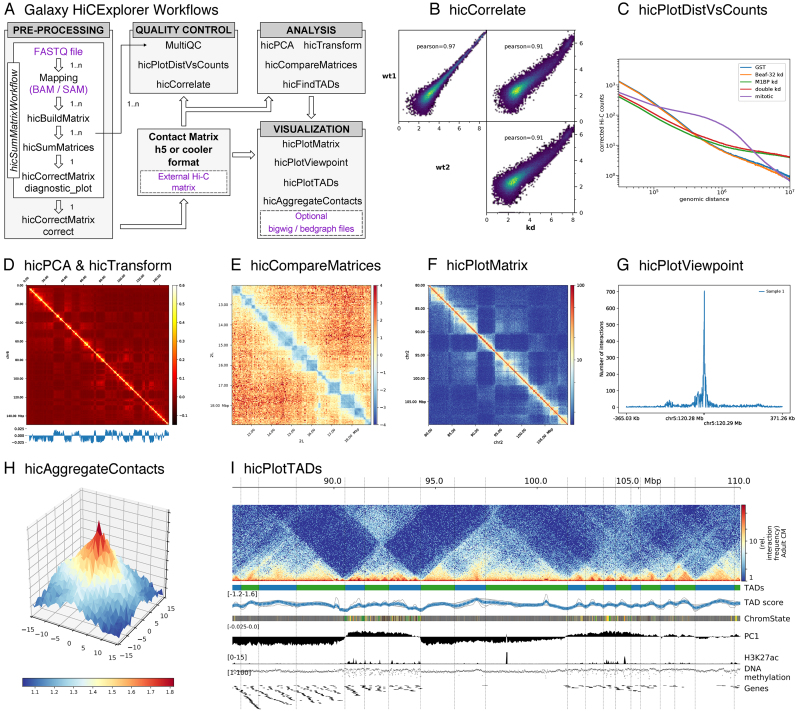
\includegraphics[scale=3.8,trim=37 0 0 45,clip]{figures/background/HiCExplorer.jpg}}
    \caption[Excerpt of HiCExplorer visualizations]
    {
        \textbf{Excerpt of HiCExplorer visualizations}
        \textbf{E)} Pixel difference computed using hicCompareMatrices and
        visualized using hicPlotMatrix of a Hi-C corrected matrix for wild type
        condition and knock down.
        \textbf{F)} Plot of a 80 to 105 Mb region contact matrix of chromosome 2 in log scale.
        \textbf{G)} Corrected number of Hi-C contacts shown using
        hicPlotViewpoint, for a single bin in chromosome 5 (output similar to
        4C-seq).
        \textbf{I)} Human chromosome 2 visualization (region 85-110 Mb) using
        tracks from different tools found in the HiCExplorer toolbox (primarily
        TAD-related information). \\
        \\Image adapted from \cite{wolff2018galaxy}.}
    \label{fig:comparison3C}\label{fig:HiCExplorer}
\end{centering}
\end{figure}





HiCExplorer \cite{wolff2018galaxy} is a collection of tools that are used to
process, analyze and visualize Hi-C data. Part of this collection are tools to
convert between formats, correcting the data (which this is work is part of),
normalizing it, analysing it in various ways, and extensively plotting it.
Facilitated is, among othters ``the creation of contact matrices, correction of
contacts, topologically associating domains (TAD) detection, A/B compartments,
merging, reordering or chromosomes, conversion from different formats including
cooler and detection of long-range contacts.''\footnotemark Those contact
matrices may then be visualized, also showing other types of data, including
``genes, compartments, ChIP-seq coverage tracks, long range contacts and the
visualization of viewpoints''\footnotemark[\value{footnote}]. An excerpt of
possible visualizations can be seen in \figref{fig:HiCExplorer}.
\footnotetext{\url{https://github.com/deeptools/HiCExplorer}, accessed 2019-06-26}



\subsection{Analysis}\label{sec:analysis}

\begin{figure}[t]
\begin{centering}
    {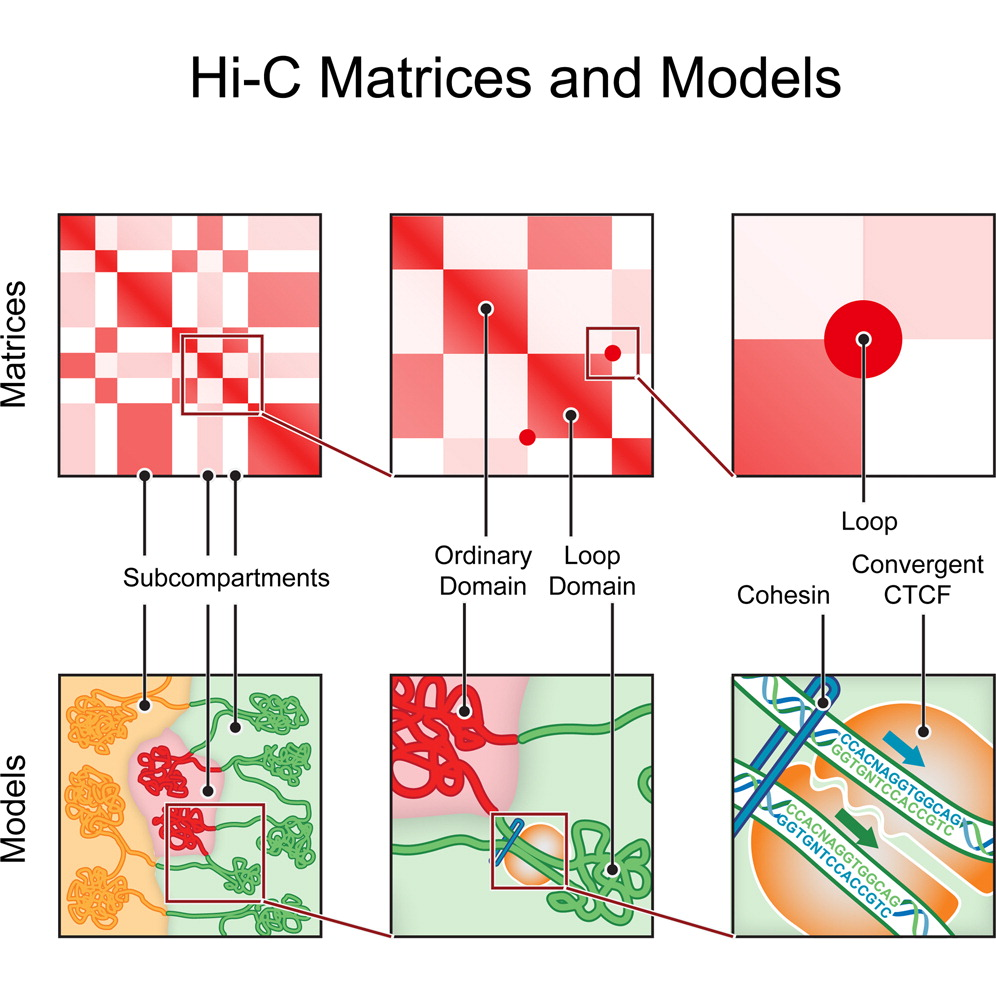
\includegraphics[scale=1.5]{figures/background/HiCMatricesModels.jpg}}
    \caption[Features revealed by HiC-Data]
    {\textbf{Features revealed by HiC-Data}.\\Image taken from \cite{rao20143d}.}

    \label{fig:HiCMatricesModels}
\end{centering}
\end{figure}




Corrected Hi-C data can then be further analysed, one such a possible further
step being to search for TADs (topologically associated domains)
\cite{ramirez2018high}, for this a TAD-seperation score is computed and local
minima indicative of TAD boundaries are searched for. A visualized result of
such a computation can be seen in \figref{fig:HiCExplorer}I. DNA is
compartmentalized \cite{lieberman2009comprehensive} in different domains, as
can be seen in \figref{fig:HiCMatricesModels}. They can be found by computing
the Eigenvectors as described in \cite{lieberman2009comprehensive} or
\cite{imakaev2012iterative} first. With this, a better understanding can be
achieved when additionally visualized. Useful metrics include difference, ratio
and log2ratio between two matrices. Replications or samples from different
conditions can easily be compared when visualized. More information about the
analysis capabilities of HiCExplorer can be found in \cite{wolff2018galaxy}.



% Analysis
%
% hicFindTADs This utility can identify TADs from a given corrected contact
% matrix by first computing a TAD-separation score and then identifying local
% minima indicative of TAD boundaries (8). In contrast to other TAD
% identification methods, this tool also returns the TAD-separation score,
% which can be visualized in a genome browser or using hicPlotTADs. The
% TAD-separation score contains useful information to identify strong and weak
% boundaries and the density of contacts within TAD and can be visualized along
% with the Hi-C matrix (see hicPlotTADs tool).
%
% hicPCA A/B compartments (1) refer to open and closed chromatin that is
% spatially separated in the cell nucleus (30,31). We compute this using
% eigenvector decomposition as described by Lieberman-Aiden (1) and using the
% first and second eigenvector. The positive/negative values correspond to
% open/closed chromatin. A visualization of A/B compartments is shown in Figure
% 1D.
%
% hicTransform The three matrices used to compute the A/B compartments
% (observed/expected, Pearson correlation and covariance matrices) are useful
% during visualization to achieve a better understanding of the Hi-C data. To
% enable this, hicTransform can compute these three matrices independently of
% hicPCA, and the matrices can then be plotted using the visualization tools.
%
% hicCompareMatrices hicCompareMatrices allows the computation of difference,
% ratio or log2ratio between two matrices. This is useful to compare replicates
% or samples from different conditions. It can, for example, help to
% characterize TAD structure modifications when followed by hicPlotMatrix
% (Figure 1E).


\subsection{Visualization}\label{sec:visualization}

% Visualization
%
% hicPlotMatrix This tool is used to plot contact matrices for a collection of
% individual chromosomes. It has multiple options to select the matrix colors
% and the values range. Additionally, bigwig tracks can be attached to plot
% additional features such as A/B compartments or ChIP-seq data. It is possible
% to plot a multitude of domains; the entire interaction matrix, individual
% chromosomes, multiple chromosomes, and various regions of interest (see
% Figure 1D–F).
%
% hicPlotViewpoint The viewpoint plot supports a visualization of the number of
% interactions around a specific reference point or region in the genome, and
% makes the long-range interactions visible as shown in Figure 1G. The output
% is comparable to what is obtained using the 4C-seq protocol.
%
% hicAggreateContacts Facilitates the analysis of long range-contacts by
% visualizing the average contacts over multiple smaller matrices around a
% given set of regions (Figure 1H).
%
% hicPlotTADs To visualize the computed TADs this tool flips the main diagonal
% of the Hi-C contact matrix by 45° and marks the TADs with triangles. It is
% possible to plot multiple matrices and add additional data like genes,
% chromatin states, long-range interactions and any other feature that can be
% represented as a bigwig or bedgraph file like methylation data, ChIP-seq, or
% RNA-seq to visually correlate them with TADs and their boundaries. There are
% multiple options to select the Hi-C matrix layout and colormap, different
% ways to visualize genes and regions files and also multiple configurations to
% plot coverage tracks like color, line width, line type, as dots, filled etc.
% (Figure 1I).


\draft{show some graphics of what analysis of such data can show}


\todo{add images here about analysis}

\todo{was kann man tun mit den visualisierungen, und auf welche wege visualisiert man das etc?  Auf welchem Wege: Z.b. mit Software des HiCExplorer: hicPlotMatrix, hicPlotTADs, hicAggregate. Die Visualisierungen braucht man um komplexere Inhalte leichter (und vor allem schnell) verstaendlich zu machen. Niemand sieht z.B. in einer Matrizen sehr schnell hoehere Zahlenwerte, als Heatmap dagegen dargestellt sieht man sofort dass da ein anderes Muster in einem Bereich ist.  }


\todo{einführung in den HiCExplorer auf die ich verlinken könnte? Siehe eine der letzten Mails da hab ich ein Paper verlinkt.}


